\documentclass{article}
\usepackage[T1]{fontenc}
\usepackage[margin=1in]{geometry}
\usepackage[french]{babel}
\usepackage{xcolor}
\usepackage{graphicx}
\usepackage{lipsum}  % produce dummy text as filler
\usepackage{array}
\usepackage{booktabs}

\newcommand\kw[1]{\textcolor{blue}{\itshape #1}}

\begin{document}

\section{Logical structure}
\subsection{Structure and visual presentation}

Some text with \emph{emphasis and \emph{nested} content}.

Some text in \textit{italic and \textit{nested} content}.

\subsection{Sectioning commands}
\subsection{Lists}

Ordered
\begin{enumerate}
  \item An entry
  \item Another One
  \item Wow! Three entries
\end{enumerate}

Unordered
\begin{itemize}
  \item An entry
  \item Another One
  \item Wow! Three entries
\end{itemize}

\section{Document classes}
\subsection{The base classes}
\begin{itemize}
  \item article
  \item report
  \item book
  \item letter
  \item slides

\end{itemize}

\section{Extending LaTeX}
\subsection{Changing how LaTeX works}

This is a lot of filler which is going to demonstrate how LaTeX hyphenates
material, and which will be able to give us at least one hyphenation point.
This is a lot of filler which is going to demonstrate how LaTeX hyphenates
material, and which will be able to give us at least one hyphenation point.

\subsection{Changing design}
\subsection{Defining commands}
Something about \kw{apples} and \kw{oranges}.

\section{Including Graphics and positioning}

This picture
\begin{center}
  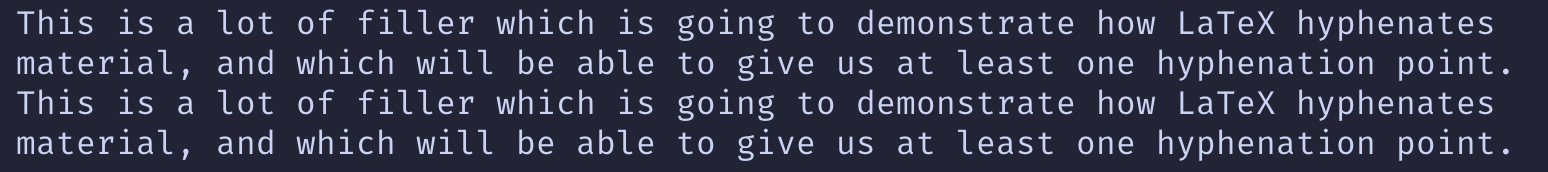
\includegraphics[width = 0.9\textwidth]{Snipaste_2023-08-23_12-30-28.png}
\end{center}
\subsection{Altering graphic appearance}

\begin{center}
  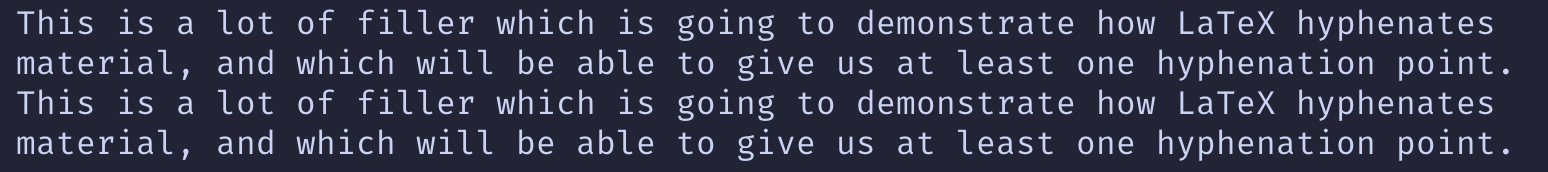
\includegraphics[height = 0.1\textwidth, width = 0.9\textwidth]{Snipaste_2023-08-23_12-30-28.png}
\end{center}
\begin{center}
  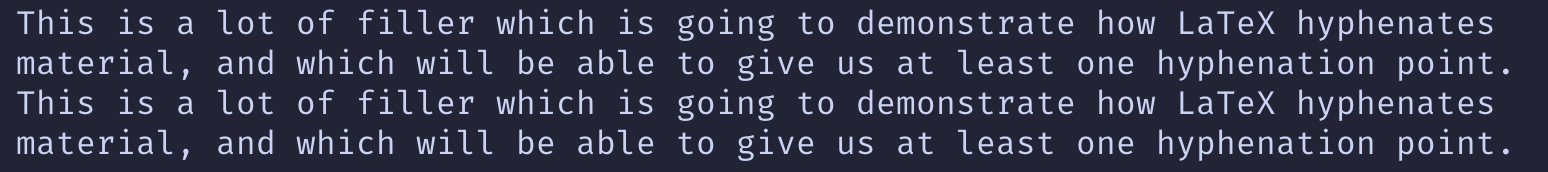
\includegraphics[clip, trim = 0 0 50 50, width = 0.9\textwidth]{Snipaste_2023-08-23_12-30-28.png}
\end{center}

\subsection{Making images float}
\lipsum[1-5] % Just a few filler paragraphs

Test location.
\begin{figure}[ht]
  \centering
  \includegraphics[width=0.5\textwidth]{example-image.png}
  \caption{An example image}
\end{figure}

\lipsum[6-7] % Just a few filler paragraphs

\section{tables}

\begin{tabular}{*{3}{l}}
  Animal & Food  & Size   \\
  dog    & meat  & medium \\
  horse  & hay   & large  \\
  frog   & flies & small  \\
\end{tabular}

\begin{tabular}{cp{9cm}}
  Animal & Description \\
  dog    & The dog is a member of the genus Canis, which forms part of the
           wolf-like canids, and is the most widely abundant terrestrial
           carnivore. \\
  cat    & The cat is a domestic species of small carnivorous mammal. It is the
           only domesticated species in the family Felidae and is often referred
           to as the domestic cat to distinguish it from the wild members of the
           family. \\
\end{tabular}

\subsection{Adding rules (lines)}

\begin{tabular}{lll}
  \toprule
  Animal & Food  & Size   \\
  \midrule
  dog    & meat  & medium \\
  horse  & hay   & large  \\
  frog   & flies & small  \\
  \bottomrule
\end{tabular}

\begin{tabular}{lll}
  \toprule
  Animal & Food  & Size   \\
  \midrule
  dog    & meat  & medium \\
  \cmidrule{1-2}
  horse  & hay   & large  \\
  \cmidrule{1-1}
  \cmidrule{3-3}
  frog   & flies & small  \\
  \bottomrule
\end{tabular}

\begin{tabular}{lll}
  \toprule
  Animal & Food  & Size   \\
  \midrule
  dog    & meat  & medium \\
  \cmidrule{1-2}
  horse  & hay   & large  \\
  \cmidrule(r){1-1}
  \cmidrule(rl){2-2}
  \cmidrule(l){3-3}
  frog   & flies & small  \\
  \bottomrule
\end{tabular}

\begin{tabular}{cp{9cm}}
  \toprule
  Animal & Description \\
  \midrule
  dog    & The dog is a member of the genus Canis, which forms part of the
           wolf-like canids, and is the most widely abundant terrestrial
           carnivore. \\
  \addlinespace
  cat    & The cat is a domestic species of small carnivorous mammal. It is the
           only domesticated species in the family Felidae and is often referred
           to as the domestic cat to distinguish it from the wild members of the
           family. \\
  \bottomrule
\end{tabular}

\subsection{Merging cells}

\end{document}



